\documentclass[]{beamer}

\usepackage[cm-default]{fontspec}
\usepackage{xunicode}
\usepackage{xltxtra}
\setmainfont[Mapping=tex-text]{DejaVu Sans}

\usepackage{graphicx}
\usepackage{amssymb}

\usetheme{Pittsburgh}
\useinnertheme{rounded}
\usefonttheme{serif}
\usecolortheme{beaver}

\title{Εισαγωγή στο Git}
\author[Σταύρος Αρώνης]{Σταύρος Αρώνης \\ \texttt{aronisstav@gmail.com}}
\date{8 Ιουνίου 2011}
\institute{Κοινότητα Ελεύθερου Λογισμικού ΕΜΠ}

\setbeamertemplate{navigation symbols}{}
\setbeamertemplate{footline}{
  \leavevmode
  \hbox{
    \begin{beamercolorbox}[wd=.5\paperwidth,ht=2.5ex,dp=1.125ex,right]
      {author in head/foot}
      \usebeamerfont{title in head/foot}
      \insertshortauthor
      \hspace{.3cm}
    \end{beamercolorbox}%
    
    \begin{beamercolorbox}[wd=.40\paperwidth,ht=2.5ex,dp=1.125ex,left]
      {title in head/foot}
      \usebeamerfont{author in head/foot}\
      \hspace{.3cm}
      \insertshorttitle
    \end{beamercolorbox}
    
    \begin{beamercolorbox}[wd=.10\paperwidth,ht=2.5ex,dp=1.125ex,center]
      {title in head/foot}
      \usebeamerfont{author in head/foot}
      \insertframenumber/\inserttotalframenumber
    \end{beamercolorbox}
  }
  \vskip0pt
}

%% \AtBeginSection[]
%% {
%%   \begin{frame}<beamer>
%%     \frametitle{Επισκόπηση}
%%     \tableofcontents[currentsection, hideothersubsections]
%%   \end{frame}
%% }

\begin{document}

\begin{frame}
  \titlepage
  \begin{center}
    
\includegraphics[height=2cm]{Fosstux.png}
    \hspace{1cm}
    
\includegraphics[height=2cm]{git-logo.png}
  \end{center}
\end{frame}

\section*{Επισκόπηση}
\begin{frame}
  \tableofcontents[hidesubsections]
\end{frame}

\section{Revision Control Systems}

\subsection{Ορισμός}

\begin{frame}
  \frametitle{Revision Control Systems}
  \begin{center}
    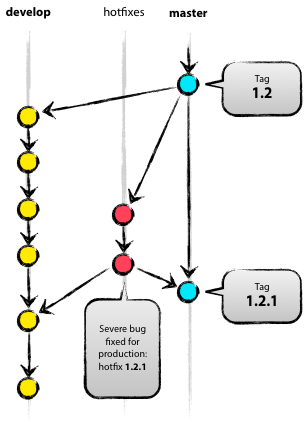
\includegraphics[height=7cm]{hotfix-branches1.png}
  \end{center}
\end{frame}

\begin{frame}
  \frametitle{Revision Control Systems}
  \begin{itemize}
    \item Χρησιμοποιούνται σε projects με πολύ κώδικα ή/και πολλούς
      collaborators.
    \item Καταγράφουν συστηματικά:
      \begin{itemize}
        \item πως
        \item γιατί
        \item ποιός και
        \item πότε
      \end{itemize}
      αλλάζει τον κώδικα.
    \item Μπορούν να χρησιμοποιηθούν αποτελεσματικά και σε εργασίες που δεν
      περιέχουν κώδικα αλλά γενικότερο text περιεχόμενο (\TeX{} documents,
      etc)
  \end{itemize}
\end{frame}

\begin{frame}
  \frametitle{Λεξιλόγιο}
  \begin{itemize}
  \item \textbf{Repository:} Το φυσικό σημείο στο οποίο βρίσκονται αποθηκευμένα
    τα αρχεία μαζί με όλες τις πληροφορίες του RCS (local ή remote).
  \item \textbf{Commit:} Ένα σύνολο λογικά συσχετιζόμενων αλλαγών στα
    παρακολουθούμενα αρχεία (edit, add, delete) μαζί με πληροφορίες για το ποιός
    τις έκανε, πότε και γιατί.
  \item \textbf{Branch:} Όταν υπάρχει ανάγκη για απόσχιση από το ``κεντρικό
    σώμα'' του κώδικα (π.χ. για ένα experimental feature ή bug fix), ένα branch
    κρατάει τα νέα commits χωρίς να επηρεάζει το σώμα του κώδικα.
  \item \textbf{Tag:} Δείκτης σε μια συγκεκριμένη έκδοση του κώδικα.
  \item \textbf{Merge:} Η διαδικασία ενσωμάτωσης ενός branch σε ένα άλλο.
  \end{itemize}
\end{frame}

\section{Distributed RCS}

\begin{frame}
  \frametitle{Distributed RCS}
  \begin{center}
    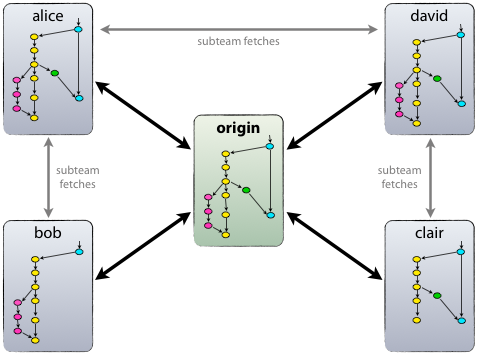
\includegraphics[height=7cm]{centr-decentr.png}
  \end{center}
\end{frame}

\begin{frame}
  \frametitle{Central RCS}
  \begin{itemize}
    \item \textbf{Βασική ιδέα:} Η ``επίσημη έκδοση'' του κώδικα βρίσκεται σε ένα
      κεντρικό repository.
    \item Κάθε commit αποθηκεύεται κεντρικά και μόνο εκεί.
      \begin{center}
        
\includegraphics[height=2cm]{social_network.jpg} \hspace{0.5em}
      \end{center}\pause
      \begin{itemize}
      \item Δεν μπορεί ο καθένας να κάνει commit.
        
\includegraphics[width=1em]{Lock1.png} \pause
      \item Πρέπει να υπάρχει σύνδεση στο δίκτυο για πρόσβαση στα commits (log,
        history, diff, blame).
      \end{itemize}
  \end{itemize}
\end{frame}

\begin{frame}
  \frametitle{Distributed RCS}
  \begin{itemize}
    \item \textbf{Δεν υπάρχει ``επίσημη έκδοση'' του κώδικα! Κάθε developer έχει
      δικό του repository!}\pause
    \item Οι collaborators έχουν \textbf{όλο} το project τοπικά:
      \begin{itemize}
        \item Κώδικας
        \item Commits
      \end{itemize}\pause
    \item Κάνουν commit τοπικά, χωρίς να επηρεάζουν κανέναν άλλο.\pause
    \item ``Πηδάνε'' από το ένα topic στο άλλο δημιουργώντας branches
      τοπικά.\pause
    \item Αξιόπιστο back-up.\pause
    \item Ανταλλάσσουν commits και συγχρονίζουν τα repositories τους.\pause
    \item Τα προβλήματα merging επιλύονται από τον developer που έκανε το patch.
  \end{itemize}
\end{frame}

\section{Git}

\begin{frame}
  \frametitle{Git}
  \framesubtitle{\url{http://git-scm.com/}}
  \begin{itemize}
  \item Projects using Git
    \begin{itemize}
    \item Git
    \item Linux Kernel
    \item Perl
    \item Eclipse
    \item Gnome
    \item KDE
    \item Qt
    \item Ruby on Rails
    \item Android
    \item PostgreSQL
    \item Debian
    \item X.org
    \item Erlang/OTP
    \end{itemize}
  \end{itemize}
\end{frame}

\begin{frame}
  \frametitle{Git}
  \begin{itemize}
    \item Κάποια από τα χαρακτηριστικά του Git:
      \begin{itemize}
        \item Εύκολο branching \pause
        \item \textbf{Εύκολο merging} \pause
        \item Έλεγχος εγκυρότητας των δεδομένων (SHA1) \pause
        \item Παρακολουθεί το περιεχόμενο συνολικά και όχι ανα αρχείο \pause
        \item Απελπιστικά γρήγορο! \pause
        \item Awesome UI \pause
      \end{itemize}
    \item Και όπως και άλλα DRCS: \pause
      \begin{itemize}
        \item Network of trust security model \pause
        \item Full access to logs and diffs
      \end{itemize}
  \end{itemize}
\end{frame}

\begin{frame}
  \frametitle{Git}
  \begin{center}
    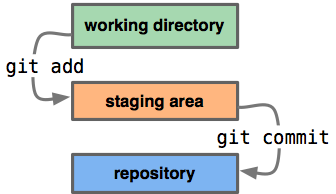
\includegraphics[width=8cm]{index1.png}
  \end{center}
\end{frame}

\begin{frame}
  \frametitle{GitHub}
  \framesubtitle{\url{https://github.com/}}
  Χρησιμεύει σαν ένα κεντρικό sync point:
  \begin{center}
    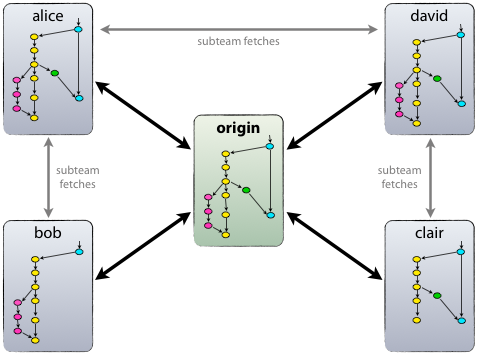
\includegraphics[height=7cm]{centr-decentr.png}
  \end{center}
\end{frame}

\begin{frame}
  \frametitle{Git Λεξιλόγιο}
  \begin{itemize}
  \item \textbf{remote:} Alias για το url ενός repository.
  \item \textbf{origin:} Κύριο remote για ένα repository που έχει δημιουργηθεί
    με clone.
  \item \textbf{master:} Default branch για ένα repository.
  \item \textbf{HEAD:} Alias για το τελευταίο commit που είναι ορατό τη δεδομένη
    στιγμή. 
  \item \textbf{SHA:} Μοναδικό αναγνωριστικό για κάθε commit.
  \end{itemize}
\end{frame}

\section{Using Git}

\begin{frame}
  \frametitle{Using Git}
  \tableofcontents[currentsection, hideothersubsections]
\end{frame}

\begin{frame}[fragile]
  \frametitle{Using Git}
  \framesubtitle{Προκαταρκτικά...}
  \begin{itemize}
    \item Στήσιμο pseudo-central server ή Λογαριασμός στο GitHub
    \item SSH keys για πιστοποίηση των collaborators
    \item Στήσιμο repository
    \item User info στο .gitconfig
\begin{verbatim}
git config --global user.name "Firstname Lastname"
git config --global user.email "your@email.com"
\end{verbatim}
  \end{itemize}
\end{frame}

\subsection{New project}

\begin{frame}[fragile]
  \frametitle{Using Git}
  \framesubtitle{New project}
  \begin{itemize}
    \item Αρχικοποίηση:
\begin{verbatim}
git init
\end{verbatim}
    \item Επισκόπηση unstaged, staged, untracked αρχείων:
\begin{verbatim}
git status
\end{verbatim}
    \item Προσθήκη αρχείων στη staging area:
\begin{verbatim}
git add <myfile.ext>
\end{verbatim}
    \item Commit των staged αρχείων στο repository
\begin{verbatim}
git commit
\end{verbatim}
    \item Καθορισμός alias για ένα remote repository:
\begin{verbatim}
git remote add <mirror> <git://github.com/foo/bar.git>
\end{verbatim}
    \item Σπρώξιμο των αλλαγών στο mirror:
\begin{verbatim}
git push <mirror> <branchname>
\end{verbatim}
  \end{itemize}
\end{frame}

\subsection{Existing project}

\begin{frame}[fragile]
  \frametitle{Using Git}
  \framesubtitle{Existing project}
  \begin{itemize}
    \item GitHub fork
    \item Δημιουργία τοπικού repository:
\begin{verbatim}
git clone <git://github.com/foo/bar.git>
\end{verbatim}
    \item Επισκόπηση αλλαγών:
\begin{verbatim}
git diff(tool)
\end{verbatim}
    \item Staging όλων των αρχείων που έχουν αλλαγές:
\begin{verbatim}
git add .
\end{verbatim}
    \item Commit με ένα απλό one-liner message:
\begin{verbatim}
git commit -m "This is a typo fix in file X"
\end{verbatim}
    \item Σπρώξιμο των αλλαγών στο mirror:
\begin{verbatim}
git push
\end{verbatim}
  \end{itemize}
\end{frame}

\subsection{Collaboration}

\begin{frame}[fragile]
  \frametitle{Using Git}
  \framesubtitle{Collaboration}
  \begin{itemize}
    \item Συγχρονισμός των local copies των remote branches:
\begin{verbatim}
git remote update
\end{verbatim}
    \item Δημιουργία τοπικού αντιγράφου από ένα τυχόν branch:
\begin{verbatim}
git fetch <git://github.com/foo/bar.git> <branch>
\end{verbatim}
    \item Ενσωμάτωση των αλλαγών:
\begin{verbatim}
git merge FETCH-HEAD
\end{verbatim}
    \item Εναλλακτικά αν οι αλλαγές είναι στο mirror του τρέχοντος branch:
\begin{verbatim}
git pull
\end{verbatim}
    \item Επίλυση conflicts μετά από failed merge:
\begin{verbatim}
git mergetool
\end{verbatim}
  \end{itemize}
\end{frame}

\subsection{Experimentation}

\begin{frame}[fragile]
  \frametitle{Using Git}
  \framesubtitle{Experimentation}
  \begin{itemize}
    \item Δημιουργία νέου branch:
\begin{verbatim}
git branch <cool_feature_name>
\end{verbatim}
    \item Εστίαση του HEAD στο νέο branch:
\begin{verbatim}
git checkout <cool_feature_name>
\end{verbatim}
    \item Δημιουργία remote branch που παρακολουθεί το νεο:
\begin{verbatim}
git push <mirror> <cool_feature_name>
\end{verbatim}
  \end{itemize}
\end{frame}

\subsection{History}

\begin{frame}[fragile]
  \frametitle{Using Git}
  \framesubtitle{History}
  \begin{itemize}
    \item Εμφάνιση του ιστορικού:
\begin{verbatim}
git log
\end{verbatim}
    \item Custom command για γρηγορη επισκόπηση ιστορικού:
\begin{verbatim}
emacs ~/.gitconfig
<< [alias]	
	tree = log --oneline --decorate --graph >>
git tree
\end{verbatim}
    \item Εμφάνιση ενός συγκεκριμένου commit:
\begin{verbatim}
git show <SHA1>
\end{verbatim}
    \item Χρήση του GUI για επισκόπηση ιστορικού:
\begin{verbatim}
gitk
\end{verbatim}
  \end{itemize}
\end{frame}

\subsection{More daily commands}

\begin{frame}[fragile]
  \frametitle{Using Git}
  \framesubtitle{More daily commands}
  \begin{itemize}
    \item Εμφάνιση branches:
\begin{verbatim}
git branch
\end{verbatim}
    \item Επισήμανση αρχείων για διαγραφή από το repository:
\begin{verbatim}
git rm
\end{verbatim}
    \item Επαναφορά του repository σε κάποιο προκαθορισμένο commit:
\begin{verbatim}
git reset HEAD
git reset <SHA1> --hard
\end{verbatim}
    \item Επαναφορά ενός αρχείου όπως εμφανίζεται σε προκαθορισμένο commit:
\begin{verbatim}
git checkout <SHA1> -- <myfile.ext>
\end{verbatim}
    \item Εμφάνιση των τελευταίων references σε commits:
\begin{verbatim}
git reflog
\end{verbatim}
  \end{itemize}
\end{frame}

\subsection{Advanced}

\begin{frame}[fragile]
  \frametitle{Using Git}
  \framesubtitle{Advanced}
  \begin{itemize}
    \item Let's find the bug:
\begin{verbatim}
git bisect
\end{verbatim}\pause
    \item Μορφοποίηση των commits:
\begin{verbatim}
git rebase -i
\end{verbatim}\pause
    \item Επιλεκτικό staging:
\begin{verbatim}
git add -i
\end{verbatim}\pause
    \item Προσωρινό καθάρισμα working space και επαναφορά:
\begin{verbatim}
git stash (pop)
\end{verbatim}\pause
    \item Εξαίρεση αρχείων από την παρακολούθηση:
\begin{verbatim}
emacs .gitignore
\end{verbatim}
  \end{itemize}
\end{frame}

\begin{frame}[fragile]
  \frametitle{Using Git}
  \framesubtitle{... having fun!}
  \begin{center}
  Git achievements \\
  \url{https://github.com/icefox/git-achievements}
\begin{verbatim}
*******************************************************
              Git Achievement Unlocked!

                       Caretaker
       Added a .gitignore file to a repository.
*******************************************************
\end{verbatim}
  \end{center}
\end{frame}

\section*{References}

\begin{frame}
  \frametitle{References}
  \begin{itemize}
    \item GitHub tutorials: \\
      \url{http://help.github.com/}
    \item Git tutorials: \\
      \url{http://www.kernel.org/pub/software/scm/git/docs/gittutorial.html}
    \item Git man pages
    \item Torvalds talk @ Google: \\
      \url{http://youtu.be/4XpnKHJAok8}
    \item Full management model using Git: \\
      \url{http://nvie.com/posts/a-successful-git-branching-model/}
    \item Git achievements
  \end{itemize}
\end{frame}

\begin{frame}
  \frametitle{Git}
    \begin{center}
      Thank you! \\
      
\includegraphics[height=4cm]{Octocat.png}
    \end{center}
\end{frame}

\end{document}

% xelatex -interaction=nonstopmode gittalk.tex; evince gittalk.pdf
